\chapter{Risultati e considerazioni}
\label{tests}
Una volta terminato lo sviluppo dell'applicazione e verificato che non ci siano
problemi durante l'esecuzione, sono stati eseguiti diversi test per verificare
correttezza e prestazione dell'applicazione.

\section{Correttezza dell'applicazione}
Per verificare la correttezza dell'applicazione si visualizza un segnale
trasformato dal programma; questo segnale \`e noto o comunque si conosce la
forma approssimativa che si dovrebbe ottenere, come accennato nel paragrafo
\ref{pyvis}. In figura \ref{fig:correctness} si vede la visualizzazione di un
segnale con larghezza di banda di 5 Mhz ed elaborato a 4096 canali di frequenza.
Come si vede dalla figura, tra i canali 1000 e 3100 circa c'\`e una grande curva
con piccoli picchi sopra di essa. La curva rappresenta il rumore introdotto
dallo strumento di misura: l'antenna, quando riceve un segnale, lo distorce in
un certo modo. Dato che questa distorsione \`e nota, \`e anche facile rimuoverla
successivamente per poter lavorare unicamente sui segnali effettivi. I picchi
presenti sopra la curva del rumore introdotto dall'antenna sono invece segnali
legittimi che possono essere studiati.
\begin{figure}[htb]
	\begin{center}
		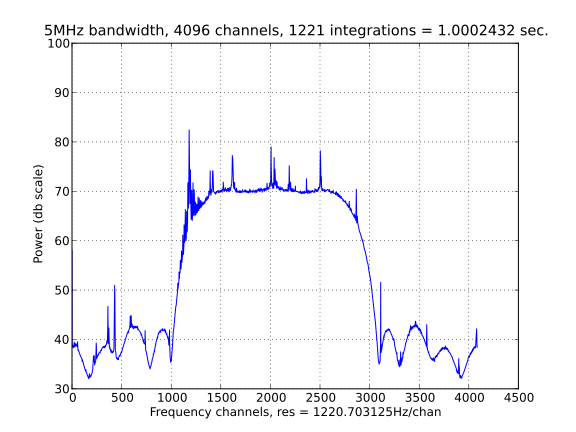
\includegraphics[width=1\linewidth]{5_4096_1221}
	\end{center}
	\caption{Visualizzazione di un segnale elaborato con il programma}
	\label{fig:correctness}
\end{figure}

Da questa immagine si capisce quindi che il programma elabora correttamente i
dati e produce una trasformazione corretta dei segnali.

\subsection{Riduzione del rumore}
Verifichiamo anche il corretto funzionamento del metodo delle somme dello stesso
segnale per attutire il rumore: nella figura \ref{fig:low_int} si vede un
segnale con 5 Mhz di banda ed elaborato a 512 canali, senza effettuare alcuna
somma di altre elaborazioni. Si pu\`o osservare con il grafico risultante sia
estremamente frastagliato e a malapena si riesce ad intuire la forma del rumore
introdotto dall'antenna, mentre gli eventuali segnali non sono nemmeno
distringuibili dal rumore di fondo.
\begin{figure}[htb]
	\begin{center}
		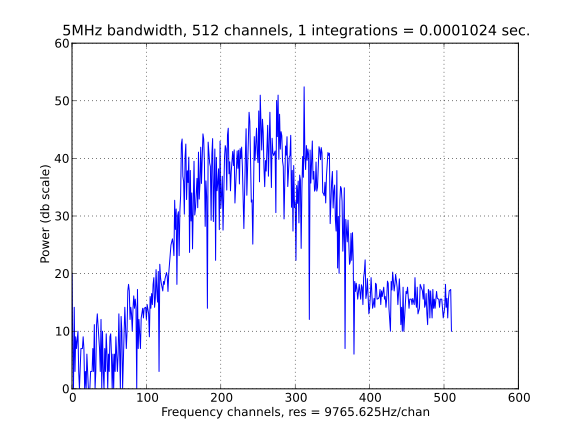
\includegraphics[width=1\linewidth]{5_512_1}
	\end{center}
	\caption{Segnale senza nessuna integrazione}
	\label{fig:low_int}
\end{figure}

Confrontiamo questa immagine con la figura \ref{fig:high_int} dove vengono
effettuate 97656 elaborazioni successive di un segnale nel tempo e poi sommate
tra di loro: in questa seconda immagine \`e perfettamente delineata la forma del
rumore dell'antenna cos\`i come sono perfettamente visibili i segnali presenti.
Si intuisce anche come le due immagini rappresentino la stessa cosa, anche se la
prima \`e un po' ``sfuocata'', non sufficientemente dettagliata, mentre la
seconda \`e molto pi\`u netta.
\begin{figure}[htb]
	\begin{center}
		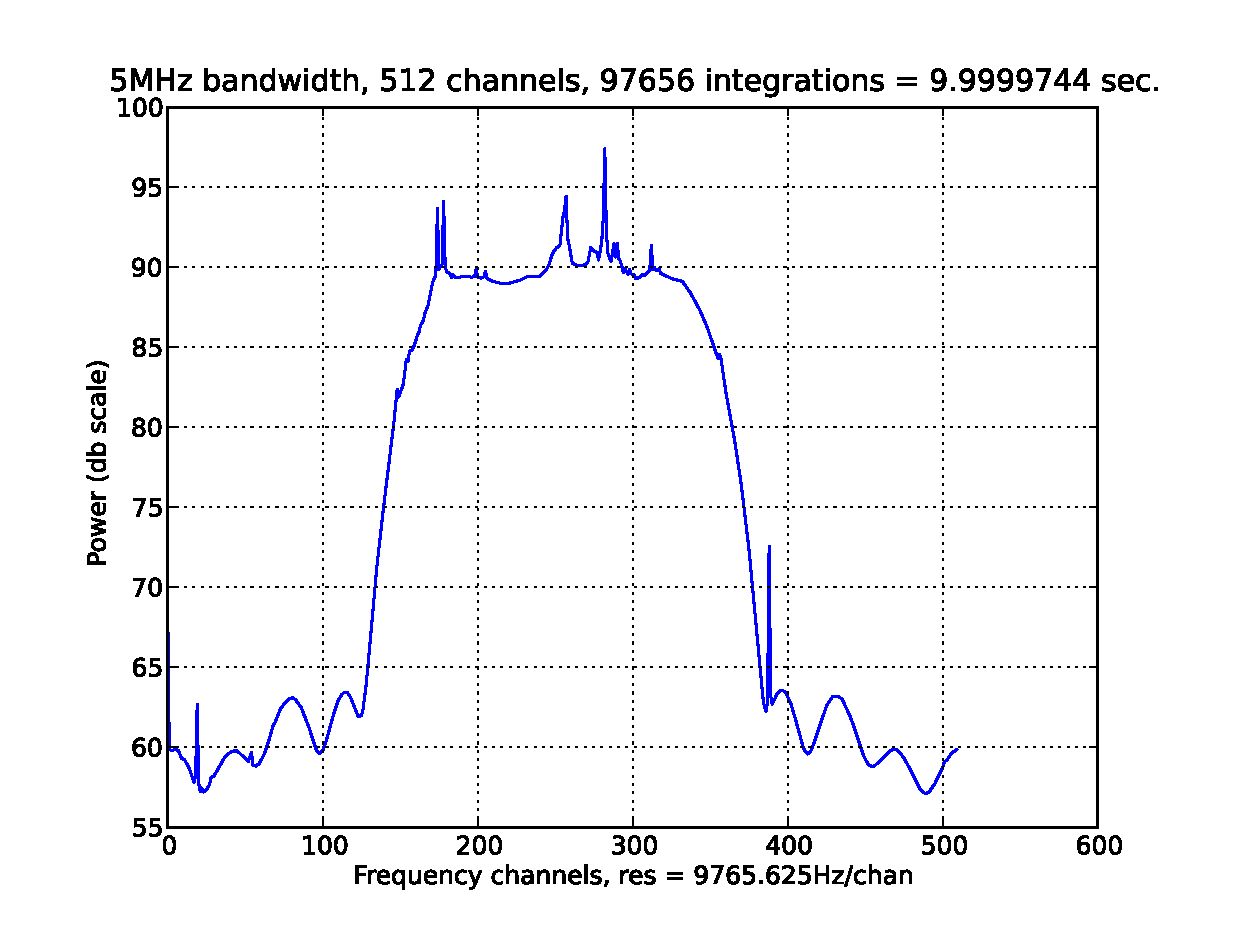
\includegraphics[width=1\linewidth]{5_512_97656}
	\end{center}
	\caption{Segnale con un elevato numero di integrazioni}
	\label{fig:high_int}
\end{figure}

Tuttavia va considerato anche che aumentando il numero di somme, aumenta anche
il tempo di elaborazione necessario: nel primo caso per calcolare i dati
rappresentati nell'immagine \`e stato richiesto un tempo di $0,00002$ secondi,
mentre nel secondo caso sono stati impiegati $2,7$ secondi.  Chiaramente va
ricercato un compromesso tra riduzione del rumore e tempo di calcolo,
compromesso che varia a seconda del tipo di analisi che si desidera fare: per
alcuni tipi di osservazioni va bene anche un segnale non molto ben definito,
purch\'e sia calcolato molto in fretta; per altri tipi di osservazioni, il
segnale deve essere definito molto precisamente, al costo di un maggiore tempo
di calcolo.

\subsection{Variazione del numero di canali}
Il numero di canali usati nel calcolo della \ac{FFT} influiscono risoluzione di
ognuno di questi canali: se i canali sono pochi, ogni canale rappresenta una
banda di frequenza piuttosto ampia, mentre con molti canali la banda di
frequenza si restringe. Aumentare il numero di canali permette di analizzare un
segnale pi\`u nel dettaglio, osservando anche variazioni tra frequenze molto
vicine tra loro. Al contrario, con pochi canali le frequenze vicine tra loro
vengono mediate. Per verificare questo fenomeno, si confrontino la figura
\ref{fig:low_chans} con la figura \ref{fig:high_chans}: nella seconda figura
tutta la zona colorata di blu \`e composta da oscillazioni vicinissime tra loro,
presenti anche nella prima figura, ma abbastanza distanziate da essere ben
visibili. Nella prima figura, ogni canale ha una risoluzione di $19531,25
Hz/canale$, mentre nella seconda ogni canale ha una risoluzione di $1,192
Hz/canale$.
\begin{figure}[htb]
	\begin{center}
		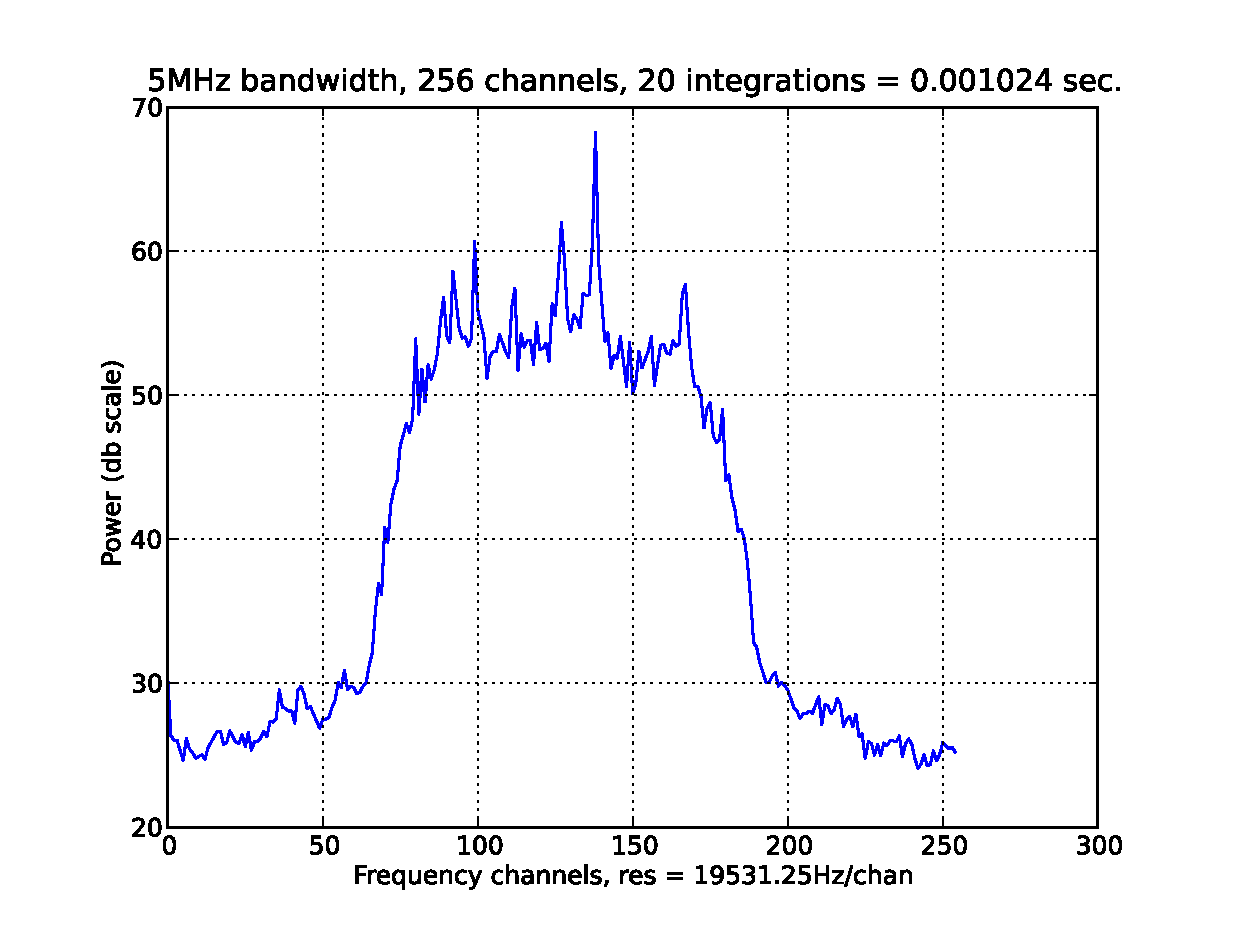
\includegraphics[width=1\linewidth]{5_256_20}
	\end{center}
	\caption{Segnale analizzato con pochi canali}
	\label{fig:low_chans}
\end{figure}

\begin{figure}[htb]
	\begin{center}
		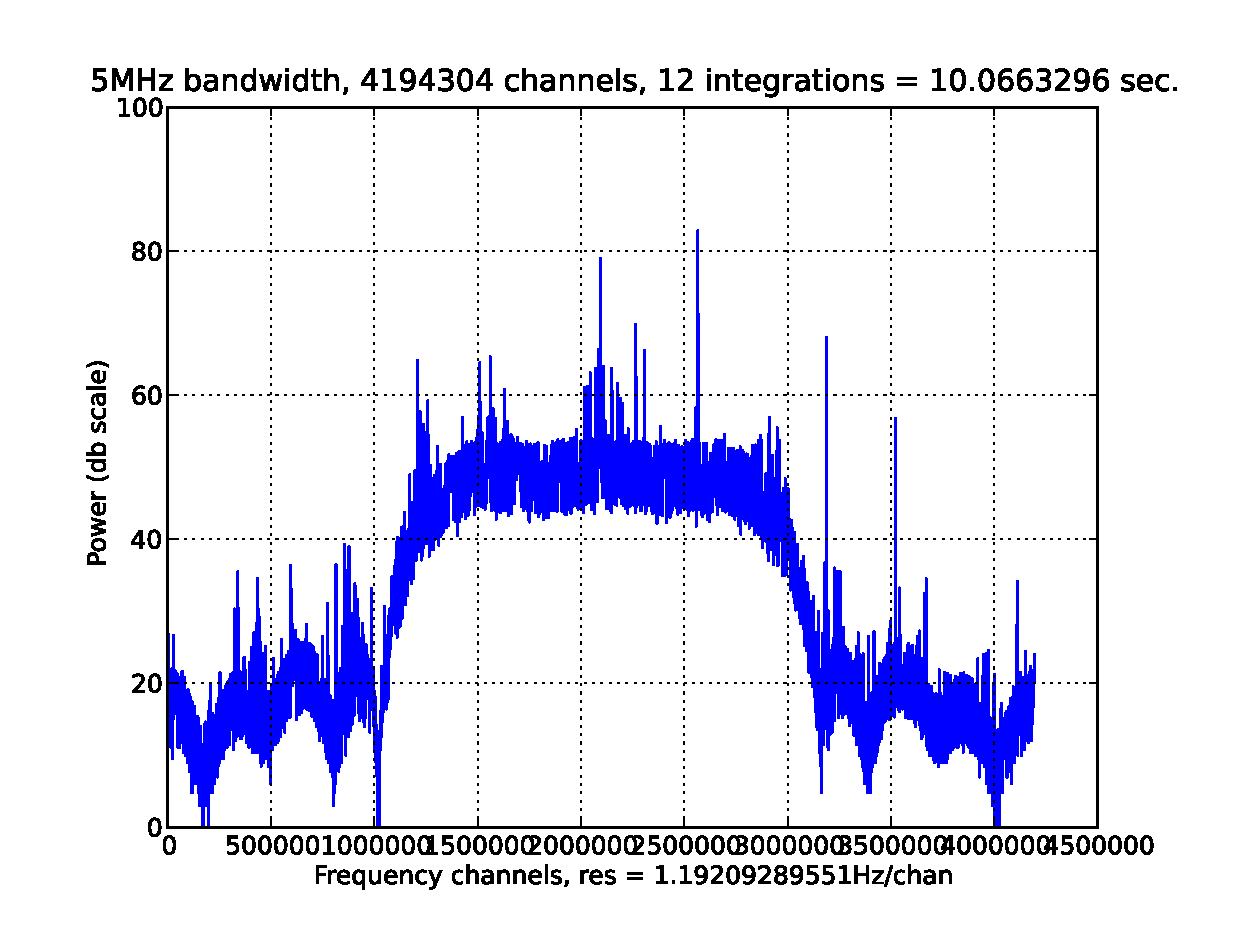
\includegraphics[width=1\linewidth]{5_4194304_12}
	\end{center}
	\caption{Segnale analizzato con molti canali}
	\label{fig:high_chans}
\end{figure}

Come per la riduzione del rumore di fondo, aumentando il numero di canali
aumenta il tempo di calcolo; allo stesso modo il compromesso tra numero di
canali e tempo di calcolo dipende dal tipo di analisi che si intende effettuare.

\section{Verifica delle prestazioni}
\ctable[
    cap=Alcuni tempi di calcolo,
    caption=Esempio di alcuni tempi di calcolo,
    label=tab:tests
]{llllll}{
\tnote[a]{Tempo espresso in secondi}
\tnote[b]{Dimensione dei files in bytes}
\tnote[c]{Si intende il tempo impiegato per effettuare tutte le \ac{FFT} e le somme dei risultati.}
}{
                \FL
Can. & Integr. & Tempo totale\tmark[a] & Dim. output\tmark[b] & Segnali output & Tempo trasf.\tmark[a]\tmark[c] \ML
256 & 1 & 4.831 & 96423936 & 94164 & 5.13041e-05\NN
256 & 20 & 5.984 & 5974016 & 5834 & 0.00102571\NN
256 & 195 & 3.952 & 403456 & 394 & 0.0100305\NN
256 & 195313 & 24.182 & 2048 & 2 & 12.091\NN
512 & 1 & 5.087 & 101545984 & 49583 & 0.000102596\NN
512 & 98 & 9.040 & 1841152 & 899 & 0.0100556\NN
65536 & 1 & 5.115 & 101974016 & 389 & 0.0131491\NN
65536 & 76 & 6.267 & 1572864 & 6 & 1.0445\NN
524288 & 1 & 3.962 & 77594624 & 37 & 0.107081\NN
524288 & 95 & 38.645 & 6291456 & 3 & 12.8817\NN
4194304 & 1 & 6.242 & 100663296 & 6 & 1.04033\NN
4194304 & 12 & 38.022 & 50331648 & 3 & 12.674\LL
}

Una volta determinato che il programma funziona, \`e stabile e produce dei
risultati corretti, si pu\`o verificare il livello di prestazioni. Per questo
sono stati fatti dei test dove si aumentava man mano il numero di canali e il
numero di integrazioni. L'aumento del numero di integrazioni \`e stato studiato
in modo che l'ordine di grandezza del tempo di calcolo previsto aumentasse ad
ogni test: se si osserva le prime righe della tabella \ref{tab:tests} si nota
che all'aumentare del numero di integrazioni il tempo si moltiplica all'incirca
per 10.\footnote{Notare che nella prima riga si impiega 20 volte meno tempo
    rispetto alla seconda. Questo perch\'e le integrazioni avrebbero dovuto
    essere 2 per ottenere un tempo 10 volte inferiore.}
Per valutare il numero di integrazioni necessarie, la formula utilizzata \`e
$integrations = \frac{bandwidth}{channels} * time$. Considerando che tutti i
segnali utilizzati hanno 5 Mhz di banda, \`e facile ricavare il numero di
integrazioni richieste. I tempi testati oscillano tra $10^-3$ e $10$.
I canali aumentano raddoppiando, per motivi visti nel paragrafo
\ref{analisi_sintesi}, e ogni volta che si incrementa il numero di canali,
conseguentemente incrementa il tempo di calcolo.

L'obiettivo di questi test \`e di verificare un eventuale limite superiore del
programma nel calcolare le trasformate. Avendo predeterminato i tempi di calcolo
desiderati, \`e facile verificare la tenuta dell'algoritmo: si osservino le
tabelle nell'appendice \ref{test_tables}, si noter\`a che tutti i tempi
rientrano nelle previsioni.
